% Edit the title below to update the display in My Documents
\title{Project Report}
%
%%% Preamble
\documentclass[paper=a4,fontsize=11pt]{scrartcl}
\usepackage[legalpaper,margin=0.7in,footskip=20pt]{geometry}
\usepackage[T1]{fontenc}
\usepackage{lmodern}
\usepackage[english]{babel}	% English language/hyphenation
\usepackage[protrusion=true,expansion=true]{microtype}	
\usepackage{amsmath,amsfonts,amsthm} % Math packages
\usepackage[pdftex]{graphicx}	
\usepackage{url}
\usepackage[natbib=true,backend=biber,bibencoding=utf8]{biblatex}
\addbibresource{references.bib}
\AtBeginBibliography{\small}

%%% Custom sectioning
\usepackage{sectsty}
\allsectionsfont{\normalfont\scshape}


%%% Custom headers/footers (fancyhdr package)
\usepackage{fancyhdr}
\pagestyle{fancyplain}
\fancyhead{}											% No page header
\fancyfoot[L]{}											% Empty 
\fancyfoot[C]{}											% Empty
\fancyfoot[R]{\thepage}									% Pagenumbering
\renewcommand{\headrulewidth}{0pt}			% Remove header underlines
\renewcommand{\footrulewidth}{0pt}				% Remove footer underlines
\setlength{\headheight}{13.6pt}


%%% Equation and float numbering
\numberwithin{equation}{section}		% Equationnumbering: section.eq#
\numberwithin{figure}{section}			% Figurenumbering: section.fig#
\numberwithin{table}{section}				% Tablenumbering: section.tab#


%%% Maketitle metadata
\newcommand{\horrule}[1]{\rule{\linewidth}{#1}} 	% Horizontal rule

\title{
		%\vspace{-1in} 	
		\usefont{OT1}{bch}{b}{n}
		\normalfont \normalsize \textsc{Building and mining knowledge graphs} \\ [25pt]
		\horrule{0.5pt} \\[0.4cm]
		\huge Assessing missing data for alternative music groups \\
		\horrule{2pt} \\[0.5cm]
}
\author{
		\normalfont 								\normalsize
        Adrian Rodriguez Grillo - 6193748\\[-3pt]		\normalsize
        \today
}
\date{}

%%% Begin document
\begin{document}
\maketitle
\section{Introduction}

Alternative or indie music was born to oppose the rules, characteristics and ways popular melodies were made, the term emerged during the 1980s and became popular in the 1990s.
In the origin, this style referred to underground bands that sound different to the mainstream rock that was prevalent in the epoch, however, nowadays the definition has become broader and affect all the existent musical genres, like pop, hip-hop, electronic, etc.

Although the sound of the songs is the main characteristic that differs from the parameters of the mainstream styles, in general, alternative bands are also identified for having different ideas and ways of how the music is produced. 
Most of these groups are out of the commercial grid and do not have much influence in scene, releasing their albums under independent records without much or any publicity and counting with his fans to make themselves known. 
Furthermore, indie groups are generally more compromised with the social context and their origin region, something that will be taken into consideration in this project.

Regarding the distribution of the music, internet has become the platform that provides the greatest revenues \cite{music_report_2018} and present a great opportunity to this type of bands to make their music known. 
The availability of complete and correct information on this platform provides a better position in searches, allowing the access to a broader audience. 
Public domain data platforms like Wikipedia \cite{wikipedia}, Wikidata \cite{wikidata}, DBpedia \cite{dbpedia} or, more specialized ones, like MusicBrainz \cite{musicbrainz} facilitates the publication of this information, however, the lack of resources of these bands leads to a situation where the data differs between websites or, directly, is missing.

\section{Problem and methodology}
A great quantity of information about alternative and underground bands exist on the internet, most of them aggregated by the fans but also by private companies that are dedicated to the music business, like Spotify \cite{spotify} or Last.fm \cite{lastfm}.
However, the data could vary in a great quantity depending of the platform visited or the search provider used, leading to inconsistencies. 

In general, these private pages contain more accurate and correct data but that is not always the case, moreover, the data is not freely available and is usually being subject to some conditions.
On the contrary, is easy to find these problems in open data portals with situations where the genres of a band differ between sites or where some information is missing in some but not others. 

In order to solve this issue, this project will study the possibility of completing the data of the open data portals using the information contained in them, this is using interlinking.
Moreover, the possibility of using external resources, like music services APIs, to complete the information will be also considered. The main objective in this project will be to complete the genre and the geographical information of the groups, however, other data will be also considered.

To accomplish the objective, the MusicBrainz dataset will be used as main source of music information, generating a knowledge graph with the data contained in the database.
This process will be done manually due to the lack of an updated dump of the data in RDF format.
The Music Ontology \cite{music_ontology} will be used as the vocabulary in order to make the data more generic and easily expandable.

The Wikidata and DBpedia knowledge graphs will be also used and linked to the data using the tools available, like the Silk framework or LIMES. Apart from the linking, the objective will be the join of the information available, filling the missing data in the correspondent sources and, generally, completing it. The GeoNames \cite{geonames} dataset is also intended to be used to give importance to the geographical information of the bands and proportionate another way of relation that could improve the discovery possibilities.

The use of external and not structured data to complete the information of the graph will be also studied. As music data is being handled, the focus will be the use of APIs of music services to complete the data in an automatic way, however, the possibility of using more unstructured sources like Wikipedia or search engines will be reviewed.

\section{Milestones and deliverables}
The main outcome of this project will be the publication of a knowledge graph that will use the MusicBrainz data as base and the Music Ontology as the main dictionary.
This knowledge graph will be linked to the data contained in Wikidata, DBpedia and GeoNames.

Additionally, a study about how is possible to tackle the completion of the data using the linked information will be assessed.
This is, how to update the content of a specific source with the knowledge contained in the linked entities, aiming for a release of a tool that performs this kind of completion.

Finally, the use of external and unstructured data to complete the information contained in knowledge graphs will be reviewed, focusing specifically in music information and the use of dedicated webservices.
The implementation of an automatic tool will be contemplated as well as a review of existent methods that perform this task.

\section{Related work, novelty and significance}
There have been previous projects that had used the MusicBrainz dataset to generate a knowledge graph in order to improve the connectivity with the linked data initiative, however they have been discontinued because of the lack of resources. 
Nevertheless, some official information exists about the process of generating a graph \cite{musicbrainz_rdf} and, also, a non-official SPARQL endpoint \cite{musicbrainz_endpoint}.

Linking knowledge graphs have been a widely covered topic and one of the main purposes of the semantic web. Tools like LIMES \cite{limes} and the Silk framework \cite{silk} facilitates the task of interlinking different knowledge graphs and in \cite{linking_book} a review all the principles related with the task can be found. Additionally, there have been some efforts to use external and unstructured information to expand and improve existent knowledge graphs \cite{completion_open, base_population, minte}.

Although in \cite{refinement_survey} the possibility of using interlinked data is contemplated to complete the knowledge graph information, the mentioned approaches effort goes into predict either missing entities, missing types for entities, and/or missing relations that hold between entities. Therefore, there is not much work that covers the problem of completing and filling the information of existent entities with data that links to them. 

Therefore, this project will build a music specific knowledge graph using techniques and methods that have been successful applied in the past to, later, improve and complete the existent data using a previously unexplored approach. 
Additionally, even though the use of external data to improve the information is not novel, using specific tools could add some value to the ecosystem.

As a passionate fan of alternative music and, specially, of small groups of my country, I think that any help this kind of groups can receive is extremely valuable for them as it increases the possibility of being discovered. 
Moreover, as a defender of open data and crowdsourced information I believe that any project that can help or give ideas on how to improve the quality of the data are extremely important nowadays. 
Specifically, if this project success it could help to improve the consistency among the different open data sources.

%%% Bibliography
{\tiny\printbibliography}

\appendix
\section{Gantt of the project}
\begin{figure}[ht]
    \centering
    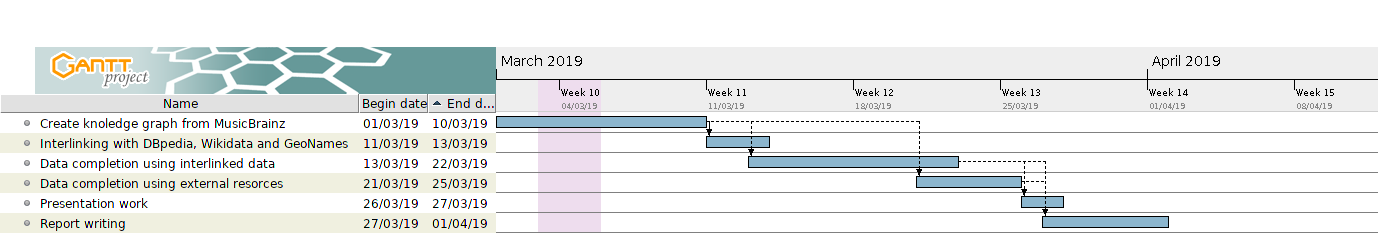
\includegraphics[angle=90,width=0.22\textwidth]{project_gantt.png}
    \caption{Gantt of the project}
\end{figure}
%%% End document
\end{document}